\documentclass[12pt]{article}
\usepackage{graphicx} % Required for inserting images
\usepackage{titling} % For custom title page
\usepackage{url}
\renewcommand{\familydefault}{\sfdefault}
\usepackage{parskip} % For spacing between paragraphs

\title{Analysing the Effectiveness of Consumer-ready Simulation Software in Training for Maritime Navigation Under Pressure}
\author{Richard Lay-Flurrie}
\date{\today}

\pretitle{
  \begin{center}
  
\includegraphics[width=0.2\textwidth]{images/logo.jpeg}\vspace{2em} \\ % Add your logo here
  \LARGE
}
\posttitle{
  \end{center}
}

\begin{document}

\maketitle
\thispagestyle{empty}

\begin{center}
  \vfill
  \large
  A thesis submitted for the degree of\\
  Doctor of Philosophy\\
  \vfill
  \normalsize
  School of Computer Science and Electronic Engineering\\
  University of Essex\\
  \vfill
\end{center}

\newpage

\section*{Acknowledgements}

Lorem ipsum dolor sit amet, consectetur adipiscing elit, sed do eiusmod tempor incididunt ut labore et dolore magna aliqua. Ut enim ad minim veniam, quis nostrud exercitation ullamco laboris nisi ut aliquip ex ea commodo consequat. Duis aute irure dolor in reprehenderit in voluptate velit esse cillum dolore eu fugiat nulla pariatur. Excepteur sint occaecat cupidatat non proident, sunt in culpa qui officia deserunt mollit anim id est laborum.

Lorem ipsum dolor sit amet, consectetur adipiscing elit, sed do eiusmod tempor incididunt ut labore et dolore magna aliqua. Ut enim ad minim veniam, quis nostrud exercitation ullamco laboris nisi ut aliquip ex ea commodo consequat. Duis aute irure dolor in reprehenderit in voluptate velit esse cillum dolore eu fugiat nulla pariatur. Excepteur sint occaecat cupidatat non proident, sunt in culpa qui officia deserunt mollit anim id est laborum.

\newpage

\section*{Abstract}

Lorem ipsum dolor sit amet, consectetur adipiscing elit, sed do eiusmod tempor incididunt ut labore et dolore magna aliqua. Ut enim ad minim veniam, quis nostrud exercitation ullamco laboris nisi ut aliquip ex ea commodo consequat. Duis aute irure dolor in reprehenderit in voluptate velit esse cillum dolore eu fugiat nulla pariatur. Excepteur sint occaecat cupidatat non proident, sunt in culpa qui officia deserunt mollit anim id est laborum.

Lorem ipsum dolor sit amet, consectetur adipiscing elit, sed do eiusmod tempor incididunt ut labore et dolore magna aliqua. Ut enim ad minim veniam, quis nostrud exercitation ullamco laboris nisi ut aliquip ex ea commodo consequat. Duis aute irure dolor in reprehenderit in voluptate velit esse cillum dolore eu fugiat nulla pariatur. Excepteur sint occaecat cupidatat non proident, sunt in culpa qui officia deserunt mollit anim id est laborum.

Lorem ipsum dolor sit amet, consectetur adipiscing elit, sed do eiusmod tempor incididunt ut labore et dolore magna aliqua. Ut enim ad minim veniam, quis nostrud exercitation ullamco laboris nisi ut aliquip ex ea commodo consequat. Duis aute irure dolor in reprehenderit in voluptate velit esse cillum dolore eu fugiat nulla pariatur. Excepteur sint occaecat cupidatat non proident, sunt in culpa qui officia deserunt mollit anim id est laborum.

Lorem ipsum dolor sit amet, consectetur adipiscing elit, sed do eiusmod tempor incididunt ut labore et dolore magna aliqua. Ut enim ad minim veniam, quis nostrud exercitation ullamco laboris nisi ut aliquip ex ea commodo consequat. Duis aute irure dolor in reprehenderit in voluptate velit esse cillum dolore eu fugiat nulla pariatur. Excepteur sint occaecat cupidatat non proident, sunt in culpa qui officia deserunt mollit anim id est laborum.

\newpage

\tableofcontents

\newpage

\listoftables

\newpage

\listoffigures

\section{Introduction}

\subsection{The Benefits of Simulation in Training}

\subsection{The Importance of Training for High-pressure Scenarios}

\subsection{Maritime Navigation Under Pressure} 

\section{Literature Review}

\subsection{Maritime Navigation Training}

In maritime navigation, the study of certain instruments and other sources of information is often required. Charts, dividers, overlays, menus, ship information, tasks lists and detailed task information may all need to be studied. \cite{atik2019use} The simulation of these instruments and sources of information in virtual environments can be achieved as seen in commercial software such as the game Stormworks: Build and Rescue \cite{stormworks} and Arma 3 \cite{arma3} (see Figure \ref{fig:tamarclassstormworks}) (see Figure \ref{fig:falklandsarma}).

\begin{figure}[h]
  \centering
  \begin{minipage}[b]{0.9\linewidth}
    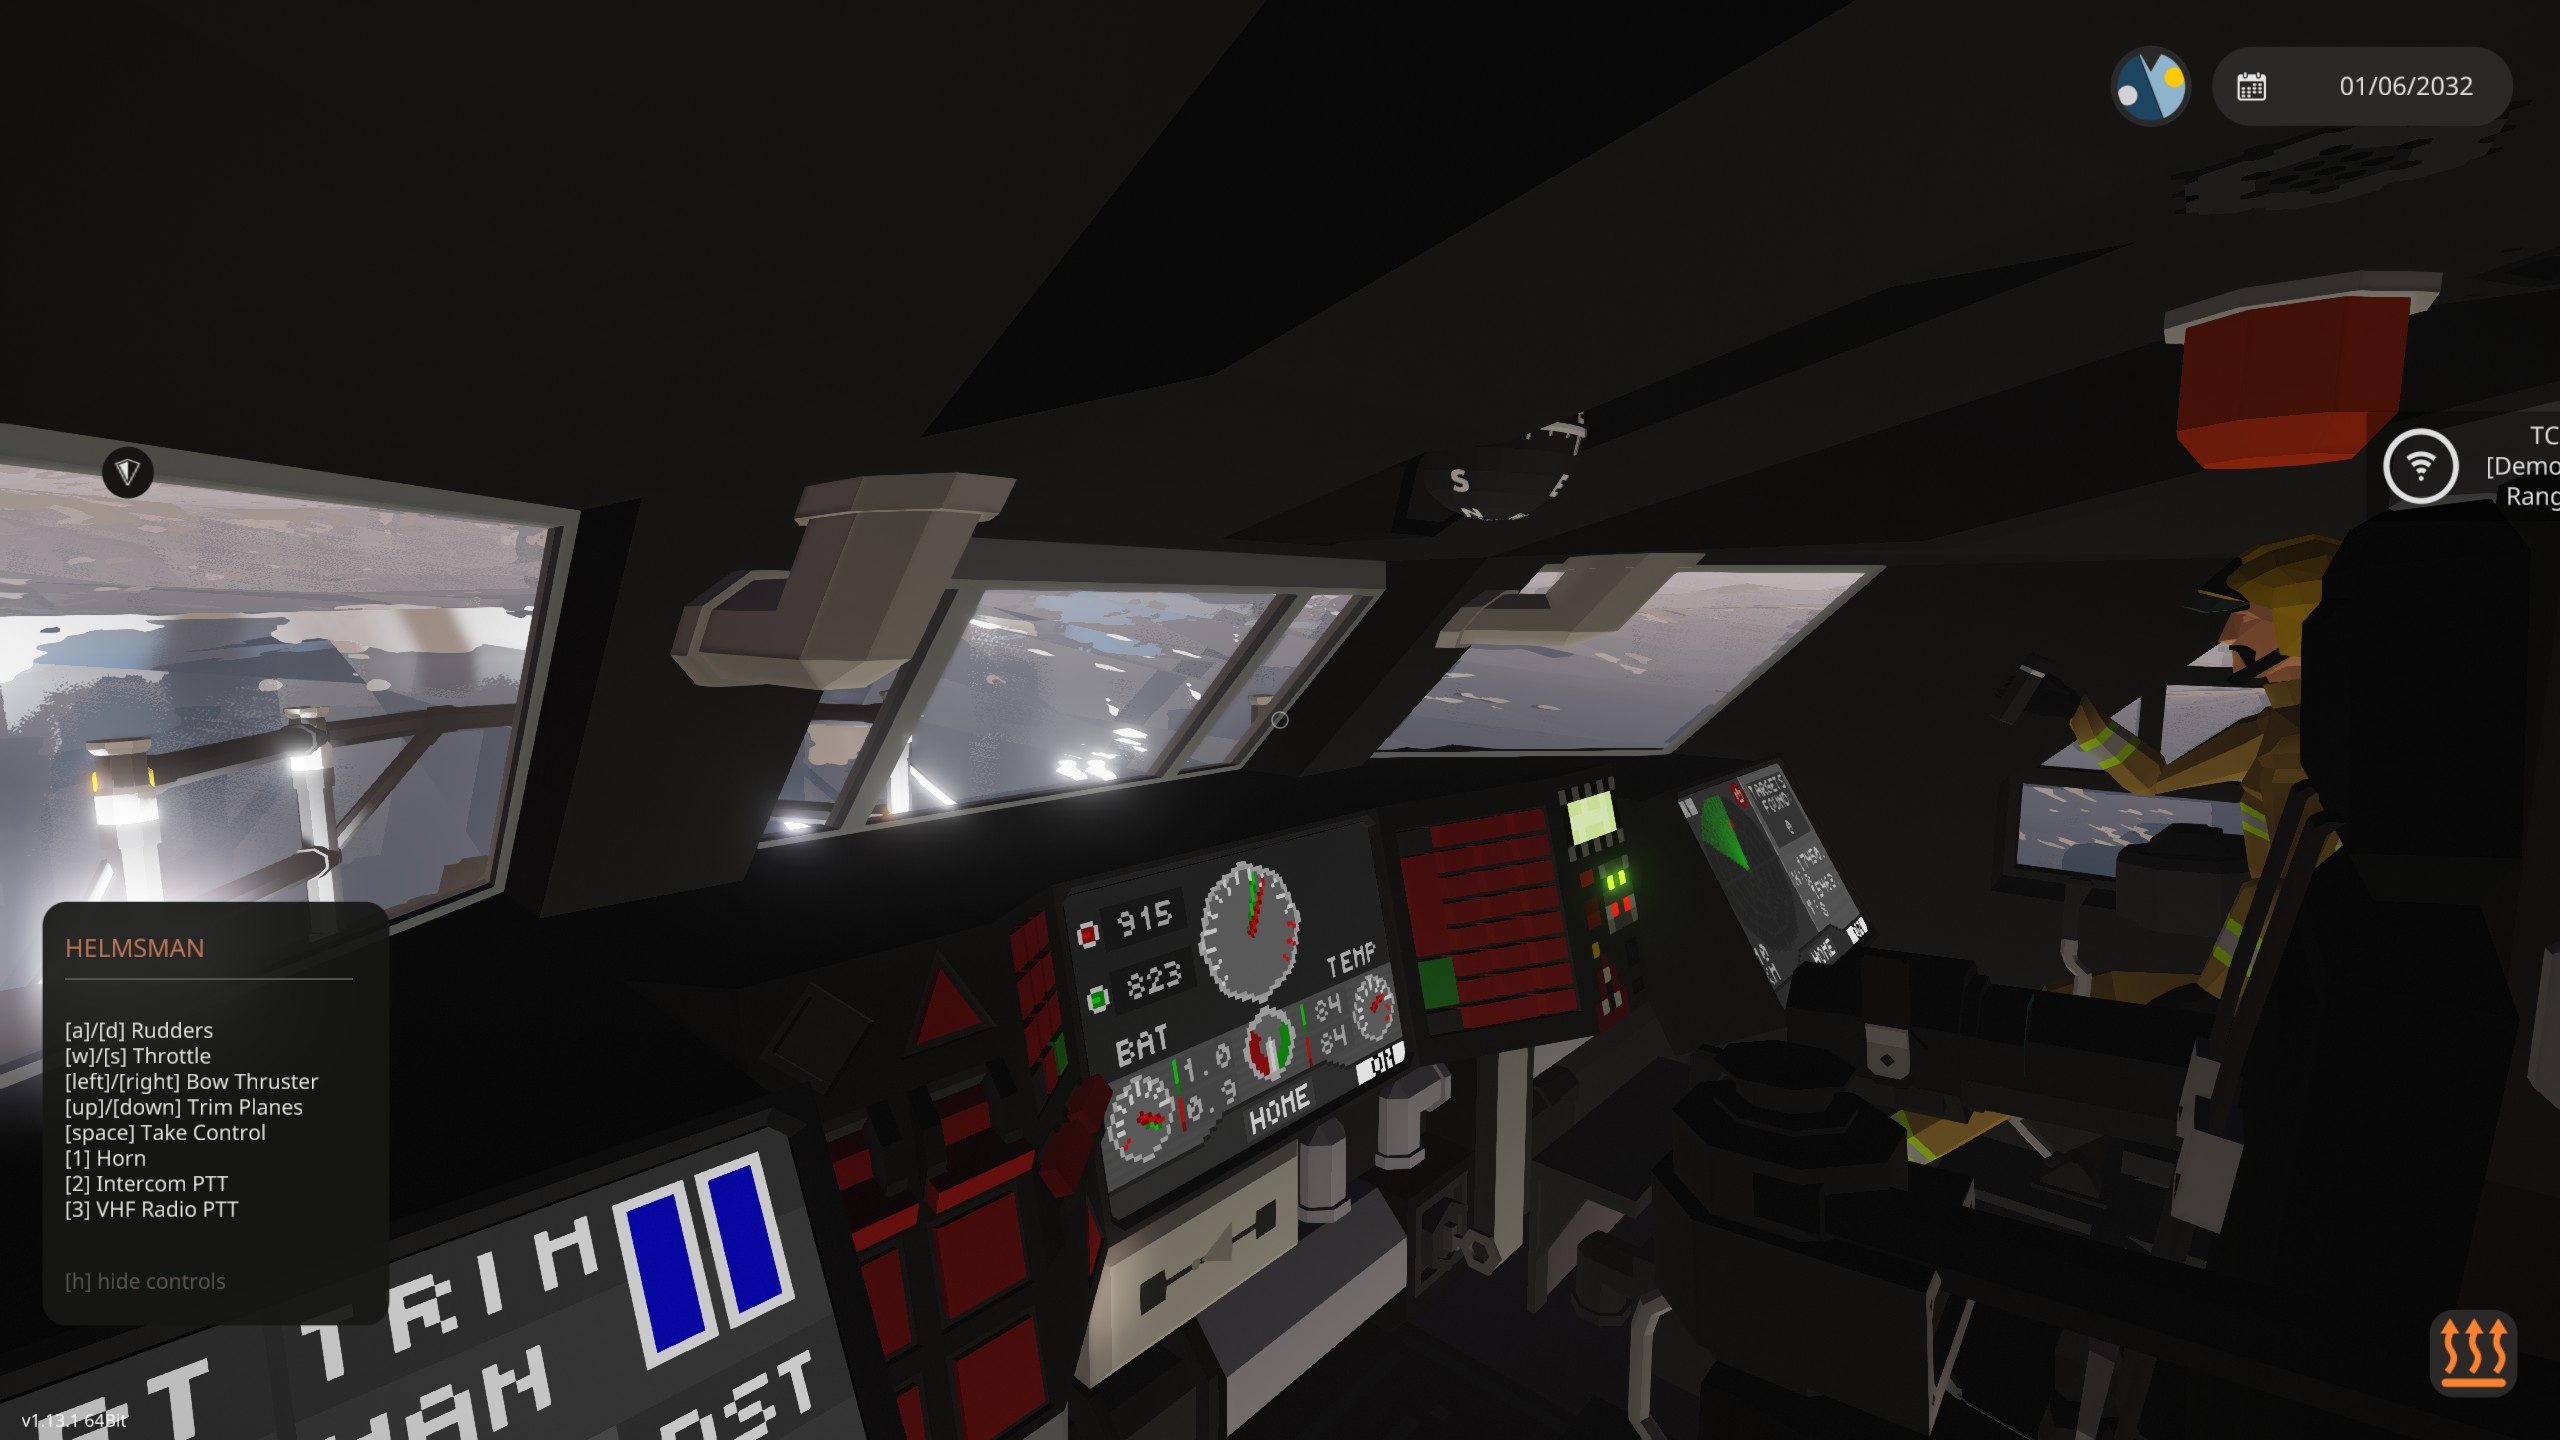
\includegraphics[width=\linewidth]{images/tamar-class-lifeboat-stormworks.jpg}
    \caption{Digital twin of a Tamar Class Lifeboat in Stormworks: Build and Rescue}
    \label{fig:tamarclassstormworks}
  \end{minipage}
\end{figure}

\begin{figure}[h]
  \centering
  \begin{minipage}[b]{0.9\linewidth}
    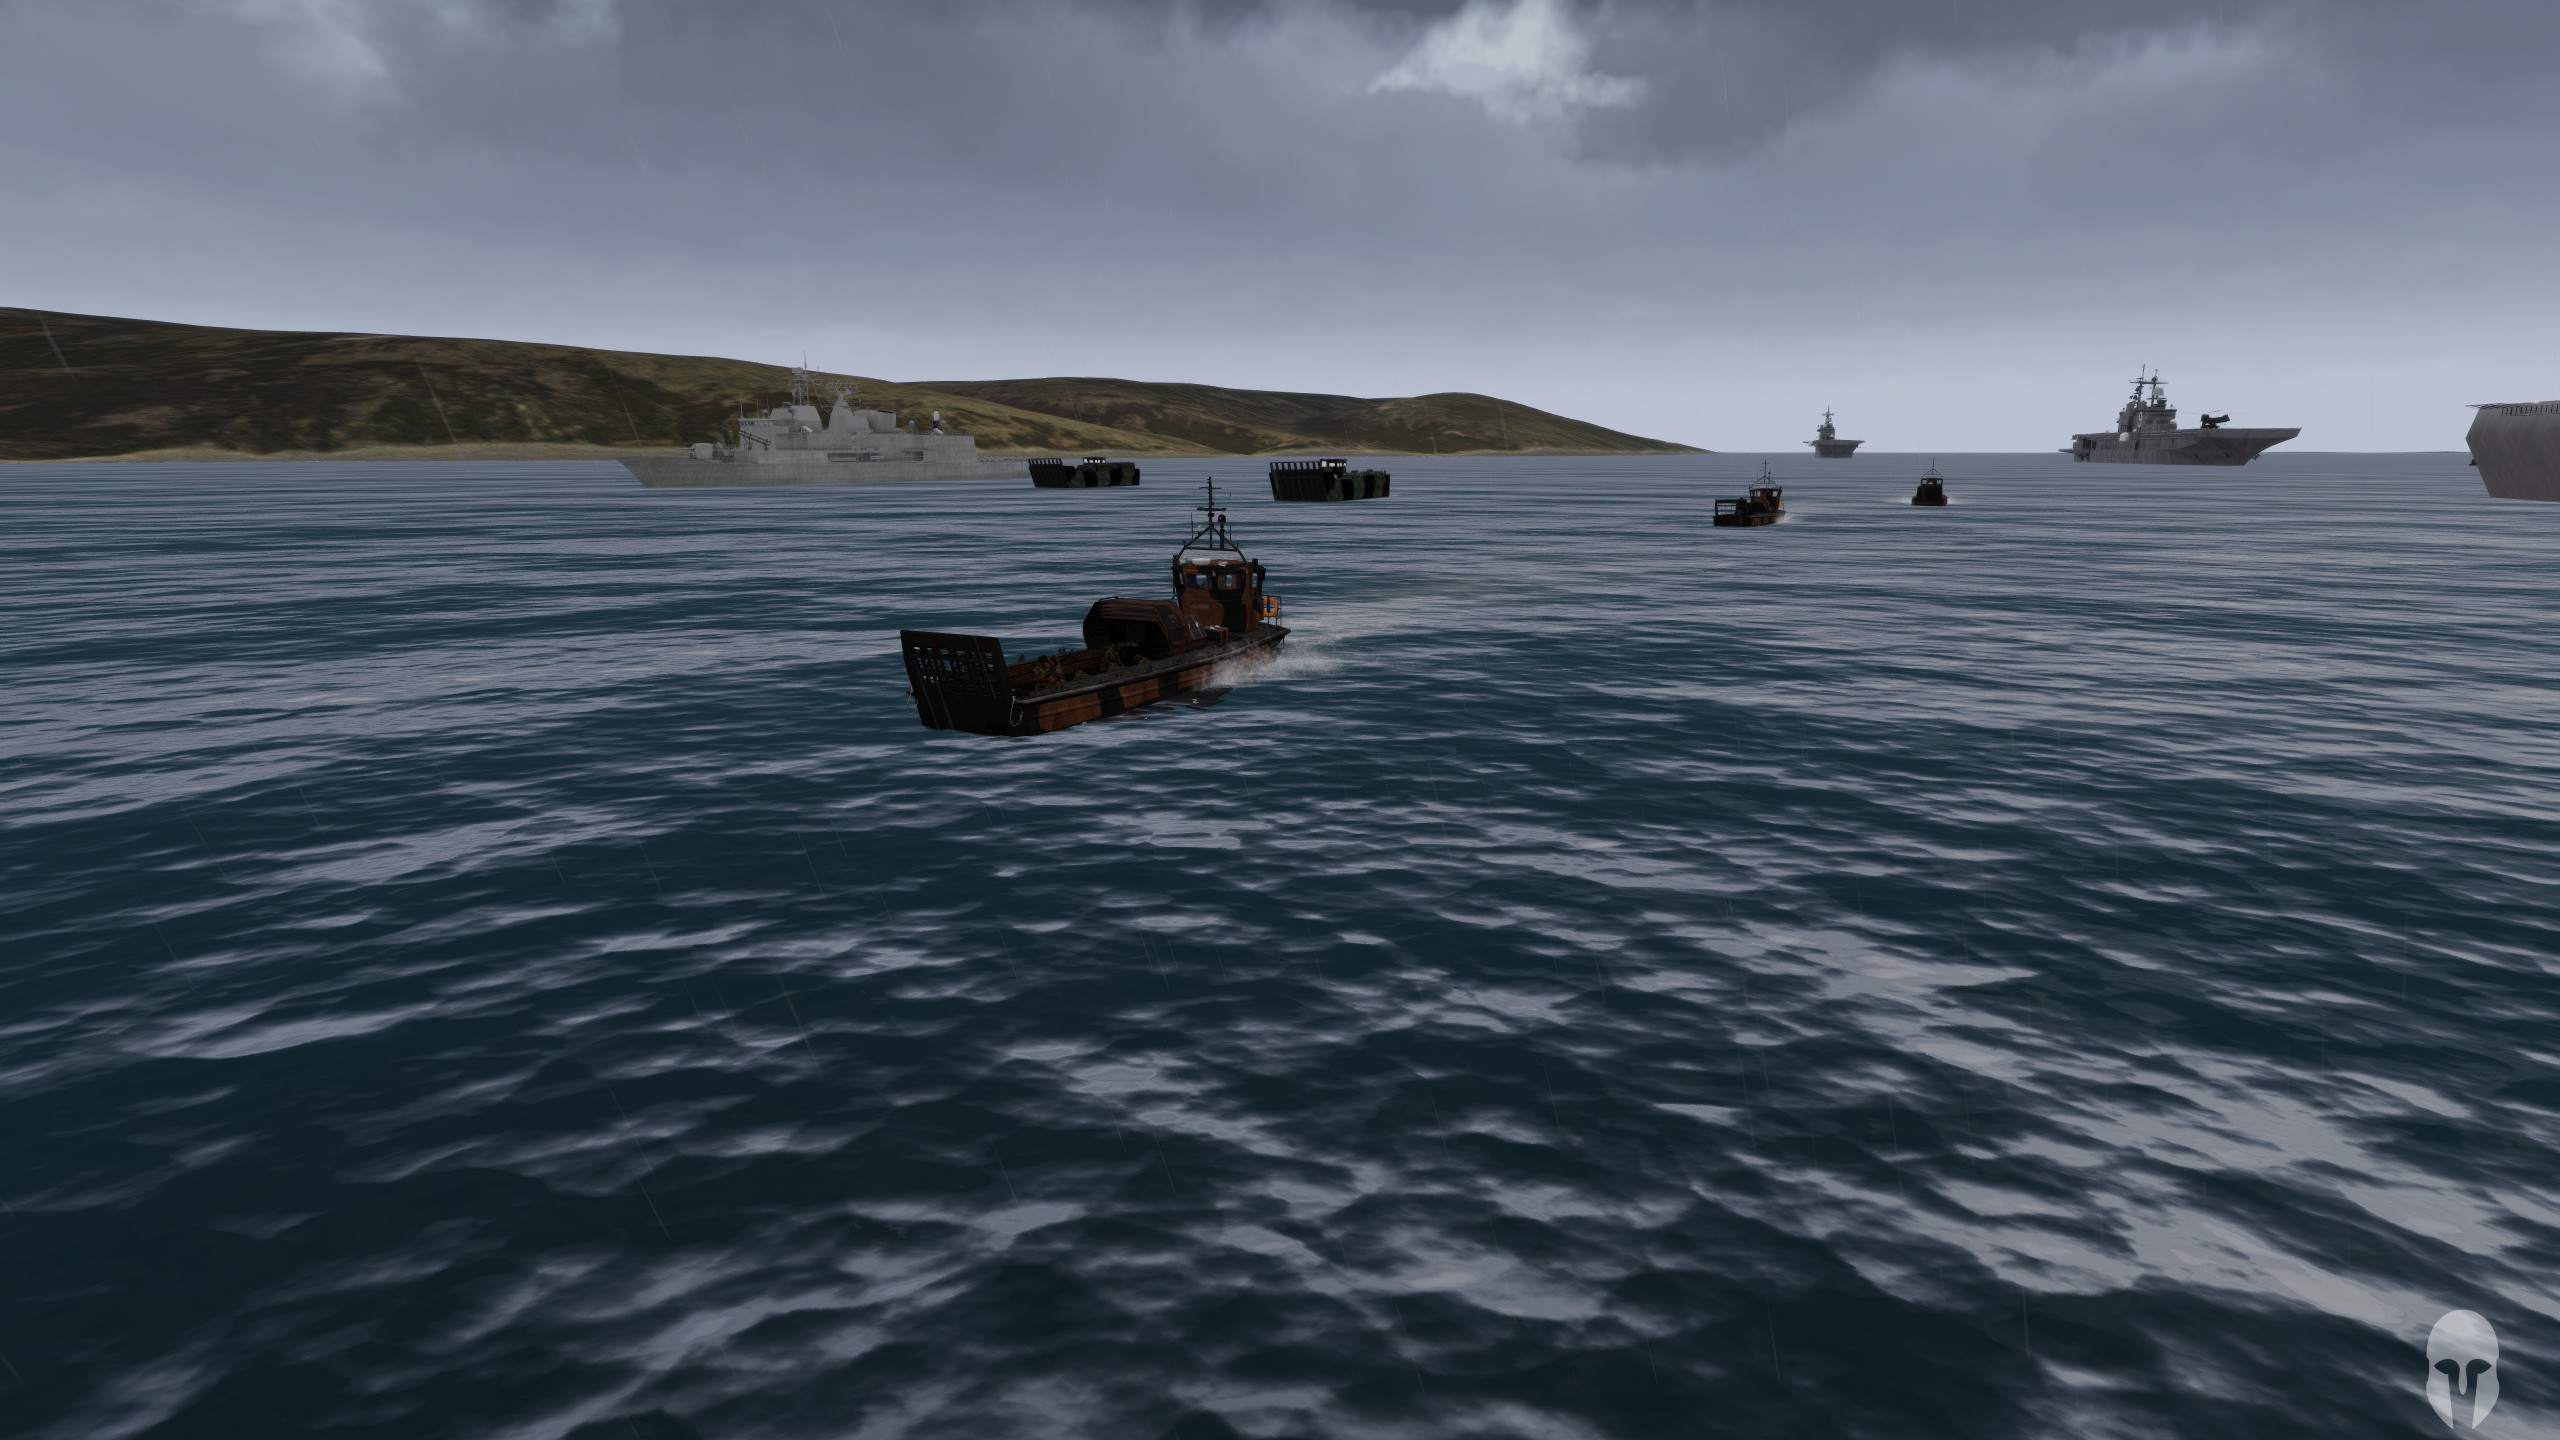
\includegraphics[width=\linewidth]{images/falklands-arma.jpg}
    \caption{Simulated Falklands War scenario in Arma 3}
    \label{fig:falklandsarma}
  \end{minipage}
\end{figure}

\subsection{High-pressure Scenarios and Decision-making}

A high-pressure situation is one which can be defined as a scenario where an invidual has a difficult task or decision to make, which is likely to make the individual feel stressed or anxious. In such situations, the individual may experience a range of physiological and psychological responses, such as increased heart rate, sweating, and impaired cognitive function. These responses can impact the individual's ability to think clearly and make effective decisions, which can have serious consequences in critical situations.

Some examples of high-pressure situations include emergencies, meeting deadlines, public speaking and competitive activities. They do not necessarily have to be life-threatening or pose a great risk to the individual to be considered high-pressure. One such example in popular media is Richie's Plank Experience \cite{richiesplank}, a virtual reality game in which the player has to walk across a plank suspended high above the ground. Although the player is not in any real danger, the immersive nature of the virtual reality experience can trigger a fear response, making it a high-pressure scenario. \cite{el2023walk}

Some factors which can contribute to the experience of stress in a situation are information overload, time pressure, complexity and uncertainty. \cite{Phillips-Wren18082020} Fear can also be considered a factor which contributes to the experience of stress. \cite{klein2013effect} Fear results from the perception of threat of danger to the person and can greatly impact decision making abilities by causing a person to focus only on things which they deem to be "catastrophic" in a given scenario. \cite{chanel2009influence} For example, in a survival situation, one may be so focused on avoiding a threat that they struggle to open a door.

\subsection{Necessity for Regular Exposure to High-pressure Scenarios}

Certain career paths require individuals to regularly make decisions under pressure such as emergency service \cite{gullon2024prevalence}\cite{smith2011work}, military \cite{srivastava2023occupational}\cite{hellewell2018measuring}\cite{fear2009job} and transport \cite{jiao2023physiological}\cite{cahill2021pilot} personnel. In these professions, the ability to think clearly and make sound decisions under pressure is critical to the safety and well-being of the individual and other people they may come in contact with or be responsible for, either directly or indirectly \cite{mcfarlane2021investigating}. 

For example, armed police officers may be required to make a decision on whether or not to deploy lethal force in a situation which is influenced by all of the aforementioned decision stressors, including fear. For many people, this is a scenario which they are unlikely to ever have to face. However, armed police officers could, in theory, have to make this decision regularly. 

\subsection{Training for High-pressure Scenarios}

Repeat exposure to the feeling of stress can help individuals to become more accustomed to it and learn how to deal with it. For this reason, military training around the world is normally designed to be stressful and, at times, unplesant. 

One such example of this is the shouting and aggression which is often used by instructors to help recruits become accustomed to thinking while under the stress of noise and unplesant attention.

As portraited in the film "Jarhead", which is based on the training of United States Marines in the early 1990s, in one scene Jake Gyllenhall's character is being slapped on the back of the head by the senior drill instructor while he is trying to recite some information. The recruit character states that he can't think while being hit on the head and the senior drill instructor retors that if he can't think while being slapped on the head, how does he expect to effectively fire his rifle in combat, an inherently stressful situation \cite{jarhead2005}.

Training for high-pressure scenarios can also take place in virtual environments. Simulations can be designed to invoke the feeling of stress in a controlled environment. A study on pilots from Fire and Emergency New Zealand found that, stress levels experienced in VR training scenarios can be very similar to those experience in the real-life scenarios. \cite{clifford2019creating}

\subsection{Application of Virtual Environments for Training}

Realistic virtual environments are ones which immerse users in a scenario by making it as close to the real thing as possible. Having access to physical objects and the use of one's own body to interact with the environment are preferred methods of immersion. \cite{clifford2018effect}

Realism can be measured both objectivly and subjectively. \cite{gonccalves2022systematic} Objective realism is the extent to which the virtual environment is similar to the real world. Subjective realism is the extent to which the user believes the virtual environment is real. Users can perceive different levels of realism in the same virtual environment. For example, some users may hone in one the graphical fidelity of the environment, while others may focus on the interactive elements such as physics and object manipulation. One study refers to a focus on the look of a virtual environment as the "fidelity trap", as it is not safe to "assume that students learn to the level of realism". \cite{carey2020high}

Realistic virtual environments can be used to effectively convey information to people in a way that is engaging and memorable. As a bonus, access to modern hardware allows for these experiences to be had at home \cite{anderson2024blending} and not require a visit to a dedicated site, which historically was the norm. \cite{Scott2022}

\subsubsection{Success in other Industries}

\subsubsection{Virtual Reality (VR)}

Virtual reality is a technology which immerses users in a virtual environment by employing hardware such as goggles, headsets, gloves or body suits to simulate the experience of "being there". This is known as telepresence. \cite{britannicaVR}

Commercially available VR devices, often used for recreation, including devices such as the Oculus series of headsets (Rift S, Quest 2) \cite{greenwald2020} can be used for training purposes. \cite{kaplan2021effects}\cite{axonVRTraining}\cite{axonVRTrainingUK}

"It's a whole new level. You know, your heart rate gets pounding. You feel emotionally invested. You start sweating and you really feel that stress and that realism that you would in that situation"

"I have never seen the sort of intense demand that we're seeing for virtual reality training." - Rick Smith AXON CEO and Founder. \cite{axonYouTube}

\subsubsection{Advandages of VR}

\subsubsection{Disadvantages of VR}

Makes people feel sick

Studies of psychological effects of long term exposure to VR

\subsubsection{Digital Twins}

A digital twin is "a virtual representation of an object or system designed to reflect a physical object accurately." \cite{ibmDigitalTwin} Digital twins are commonly found in video games with the primary use being for recreation. Digital twins of real world items are especially prevalent in games which replicate the real world. For example, aircraft and naval assets in Digital Combat Simulator World \cite{dcsworld}, vehicles in the racing simulation iRacing \cite{iracing} or weapons in the first person shooter series Battlefield \cite{battlefield4}. However, digital twins can also be used for training purposes such as in the logistics industry \cite{longo2023prepare} and in the military \cite{ukcatt}.

Digital twins provide a key benefit to training in virtual environments in that they can be used to demonstrate how a physical object or system works and allow a user to experiment with it in a controlled environment. For example, a digital twin of a ship's bridge can be used to train maritime navigation students on how to use the equipment in a safe environment. 

Digital twins do also have limitations in that, if not implemented accurately, they can provide unrealistic expectations of the real thing. During a demonstration of a proposed animatronic doll for a project, Youtuber Michael Reeves demonstrates how the digital twin can rotate its jaw through 360 degrees. (see Figure \ref{fig:michaelreeves}) "Uhh, ooo, can't do that in real life" he says. \cite{reevesYouTube}

\begin{figure}[h]
  \centering
  \begin{minipage}[b]{0.9\linewidth}
    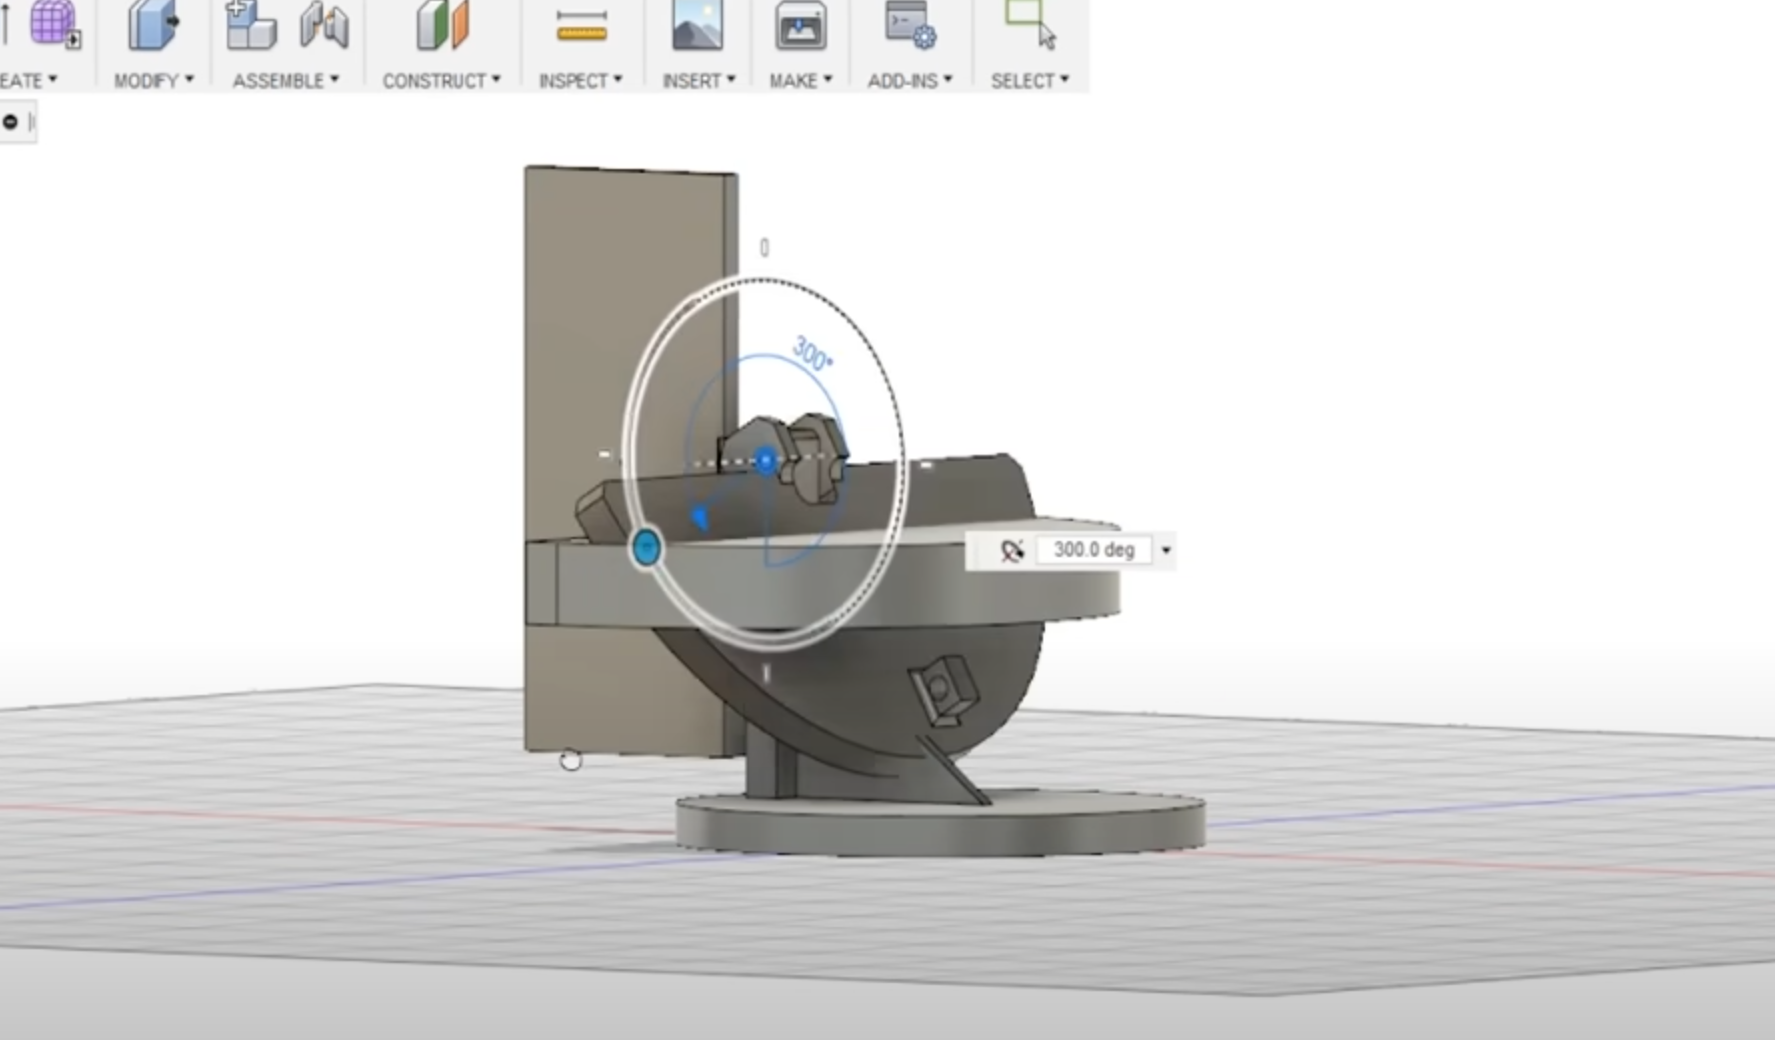
\includegraphics[width=\linewidth]{images/michael reeves.png}
    \caption{Digital twin of an animatronic doll rotating its jaw through 360 degrees}
    \label{fig:michaelreeves}
  \end{minipage}
\end{figure}

\subsection{Creating Realistic Virtual Environments}

\subsubsection{Key Design Princples}

\subsubsection{Defining Realism}

\subsubsection{Generation of HDRI Backdrops}

\subsubsection{Photogrammetry}

\subsubsection{3D Printing}

\subsubsection{Tactile Models to Support Training in Virtual Environments}

\subsection{Measuring Stress Levels}

Data regarding the stress level of a participant can be attained by measuring a person's heart rate, heart rate recovery time, salivary cortisol and amylase. Further surveys and interviews can be conducted with volunteers to gather information. \cite{liu2018impact}

Eye-tracking solutions may also be used to measure stress levels in the same way as they have been used to measure competency in martitime navigation training. \cite{atik2019use}

\subsection{Application of Virtual Environments in Training for High-pressure Scenarios} \label{sec:applicationsOfVirtualEnvironments}

Training for high-pressure scenarios can be expensive and dangerous. From 1st January 2000 to 29th February 2024, 162 UK armed forces personnel died whilst on training or exercise. \cite{ukmod2024} In a report published by the UK Ministry of Defence, the cost of 105mm artillery shells between the commencement of Operation Herrick 17 and 17th December 2014 ranged from ~£50.00 to ~£2,812.00 per shell, depending on the type of shell and other factors. \cite{ukmod2015} Assuming a cost of £50.00 per shell (at the lower end of the scale), the cost of a battery of 6 guns firing 6 shells each, per fire mission, would be £1,800.00. This is a significant cost for a single training exercise which could potentially last weeks or more. Now scale this up to the cost of a year's worth of training for the entire UK armed forces and the cost becomes astronomical. For example, exercise Steadfast Defender involved ~90,000 troops and personnel, 50+ naval assets, 80+ air platforms and over 1,1000 combat vehicles. \cite{steadfastdefender24}

In 2024, an Apache helicopter deployed on an exercise in Jordan with the Utah National Guard crashed. \cite{intergalactic2024} No one was killed in the crash but the cost of the aircraft, as of the date of the crash, was around 50 million USD. \cite{cbsaustin2024} It is theorised that the crash was caused by an experiened jet pilot attempting to control the rotary wing aircraft and causing an irrecoverable stall. \cite{carlisle2024}

On the 13th of January, 2024, the 47th Separate Mechanized Brigade of the Ukrainian Army reported the destruction of a Russian T-90 Proryv tank. \cite{malyasov2024} It has been proven that the T-90's external systems (such as optics) were destroyed by the main cannon of a Bradley AFV, commanded by Serhiy of the Ukrainian Army. In an interview with Serhiy, he stated that he knew which parts of the tank to fire at (to damage the external systems) as he had practised in "video games" \cite{militaryconflict2025} (it is likely, although unconfirmed, that he is referring to War Thunder \cite{warthunder}).

University students can undertake courses in maritime operations and technology, such as the one offered by the University of South Eastern Norway. They can use a ship bridge simulator to practice their skills in a controlled environment as seen in Figure \ref{fig:maxvdhnorway}.

\begin{figure}[h]
  \centering
  \begin{minipage}[b]{0.9\linewidth}
    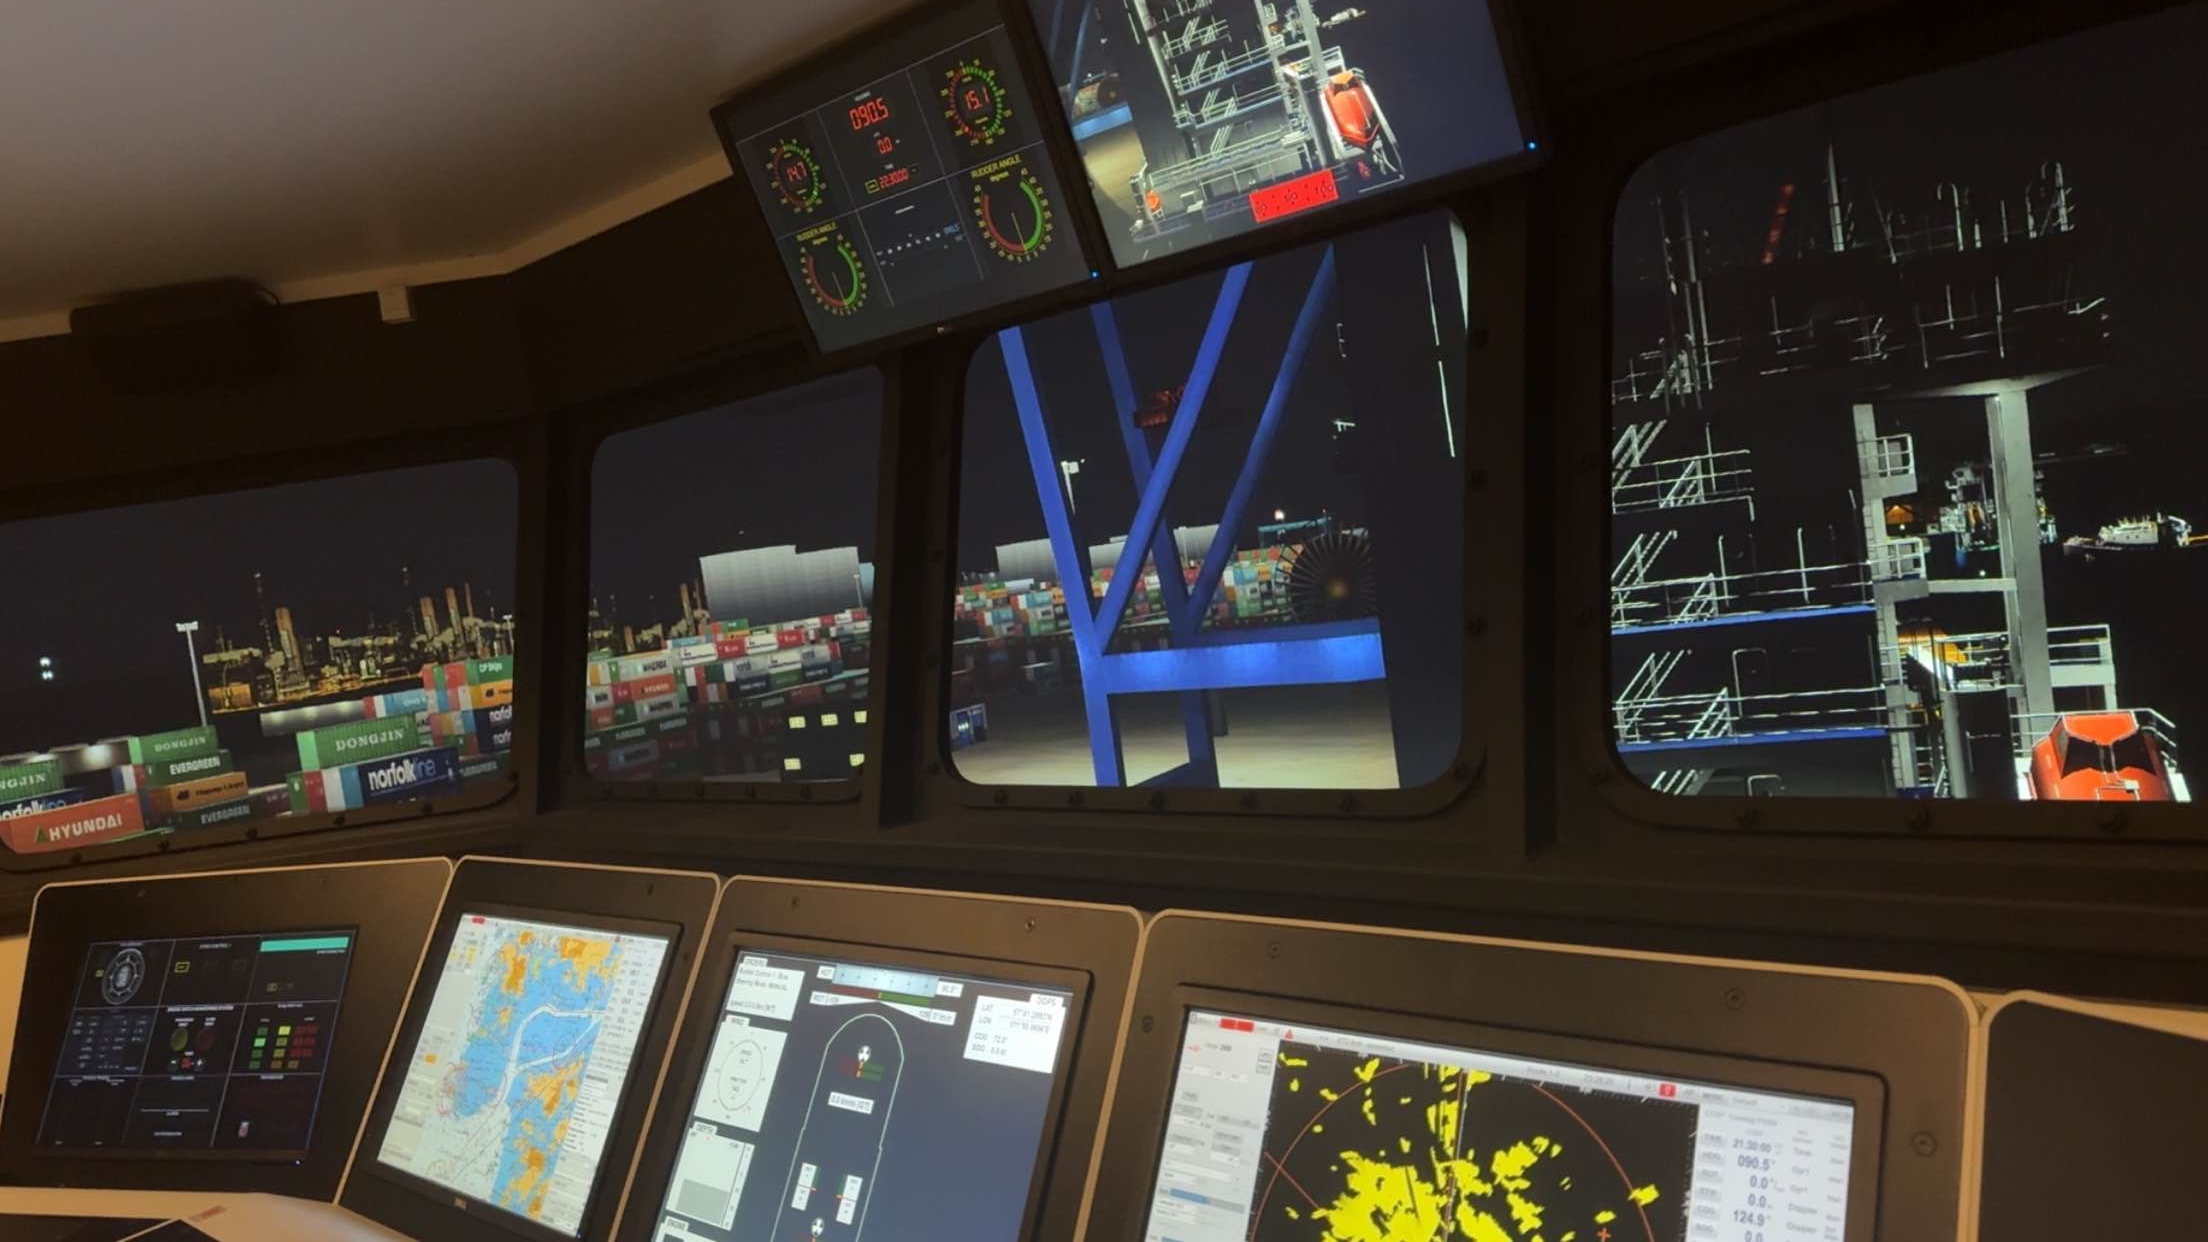
\includegraphics[width=\linewidth]{images/max_vdh_norway.jpg}
    \caption{A simulated ship bridge simulator, with screens and physical controls, at the University of South Eastern Norway courtesy of Max Van Der Haagen, student.}
    \label{fig:maxvdhnorway}
  \end{minipage}
\end{figure}

\subsection{Challenges with Maritime Experimentation}

% https://journals.plos.org/plosone/article/file?id=10.1371/journal.pone.0186871&type=printable

\subsubsection{Gathering Data}

Ensuring accuracy and reliability

\subsubsection{Minimising Risk}

\subsubsection{Logistics}

\subsubsection{Ethical Considerations}



\subsection{Preparation for Experiments in Potentially Dangerous Situations}

\subsubsection{Gathering Data}

Privacy Concerns

\subsubsection{Minimising Risk}

Ensuring people are comfortable with water and understanding how to stay safe in water

Intake questionairres 

Apparatus

\subsection{Preparation for Maritime Experimentation}

\subsubsection{Volunteers}

Intake questionairres 

\subsubsection{Apparatus}

Apparatus

\subsection{Performance Measures}

https://www.taylorfrancis.com/chapters/edit/10.4324/9781315243092-21/performance-measurement-simulation-based-training-eduardo-salas-michael-rosen-janet-held-johnny-weissmuller

\subsubsection{Simulation}

\subsubsection{Real-world}

\subsection{Preparation for Simulator Experimentation}

\subsubsection{Volunteers}

Selection and Training of Participants

\subsubsection{Apparatus}

\subsection{Consumer-ready Simulation Software}

\subsection{Data Collection}

\subsubsection{Simulation}

\subsubsection{Real-world}

\section{Building Virtual Environments for Training in Unreal Engine 5}

\subsection{Introduction}

\subsection{Digital Twins}

\subsection{Unreal Engine 5}

\section{Human Perception and Differentiation of Real and Virtual Environments}

\subsection{Introduction}

\subsection{Methodology}

\subsection{Experiment 1 - Mutilus}

\subsubsection{What is Mutilus?}

\subsubsection{Prototype Experiments}

\subsubsection{Results}

\section{Applications of this Research}



\subsection{Training for Stressful Scenarios}

\section{Methodology}

\section{Results}

\section{Discussion}

\section{Conclusion}

\section{References}

\bibliographystyle{ieeetrans}
\bibliography{references}

\section{Appendices}



\end{document}
